\documentclass[border=5pt]{standalone}
\usepackage{tikz}
\usetikzlibrary{shapes, positioning, arrows.meta, fit, backgrounds}

\begin{document}
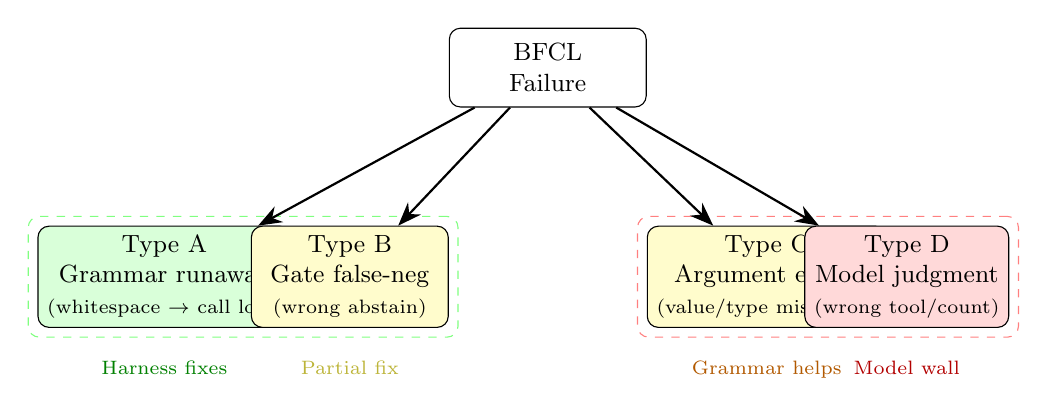
\begin{tikzpicture}[
  node distance=1.2cm,
  box/.style={draw, rounded corners, align=center, font=\small, minimum width=2.5cm, minimum height=1cm},
  fixed/.style={box, fill=green!15},
  partial/.style={box, fill=yellow!20},
  wall/.style={box, fill=red!15},
  label/.style={font=\scriptsize, text=gray},
  arrow/.style={-{Stealth[length=3mm]}, thick},
]

% Root
\node[box] (root) {BFCL\\Failure};

% Level 1
\node[fixed, below left=1.5cm and 2cm of root] (a) {Type A\\Grammar runaway\\{\scriptsize (whitespace $\to$ call lost)}};
\node[partial, below left=1.5cm and 0cm of root] (b) {Type B\\Gate false-neg\\{\scriptsize (wrong abstain)}};
\node[partial, below right=1.5cm and 0cm of root] (c) {Type C\\Argument errors\\{\scriptsize (value/type mismatch)}};
\node[wall, below right=1.5cm and 2cm of root] (d) {Type D\\Model judgment\\{\scriptsize (wrong tool/count)}};

\draw[arrow] (root) -- (a);
\draw[arrow] (root) -- (b);
\draw[arrow] (root) -- (c);
\draw[arrow] (root) -- (d);

% Harness scope
\node[below=0.3cm of a, font=\scriptsize, text=green!50!black] {Harness fixes};
\node[below=0.3cm of b, font=\scriptsize, text=yellow!70!black] {Partial fix};
\node[below=0.3cm of c, font=\scriptsize, text=orange!70!black] {Grammar helps};
\node[below=0.3cm of d, font=\scriptsize, text=red!70!black] {Model wall};

% Scope box
\begin{scope}[on background layer]
\node[draw=green!50, dashed, rounded corners, fit=(a)(b), label={[font=\scriptsize, green!50!black]below:Harness-recoverable (form)}] {};
\node[draw=red!50, dashed, rounded corners, fit=(c)(d), label={[font=\scriptsize, red!50!black]below:Model-limited (judgment)}] {};
\end{scope}

\end{tikzpicture}
\end{document}
